\begin{frame}{optimizing real programs}
    \begin{itemize}
    \item ask your compiler to try first
    \vspace{.5cm}
    \item spend effort where \myemph{it matters}
    \item e.g. 90\% of program time spent reading files, but optimize computation?
    \item e.g. 90\% of program time spent in routine A, but optimize B?
    \end{itemize}
\end{frame}

\begin{frame}{profilers}
    \begin{itemize}
    \item first step --- tool to determine where you spend time
    \item tools exist to do this for programs
    \item example on Linux: \texttt{perf}
    \end{itemize}
\end{frame}

\begin{frame}{example}
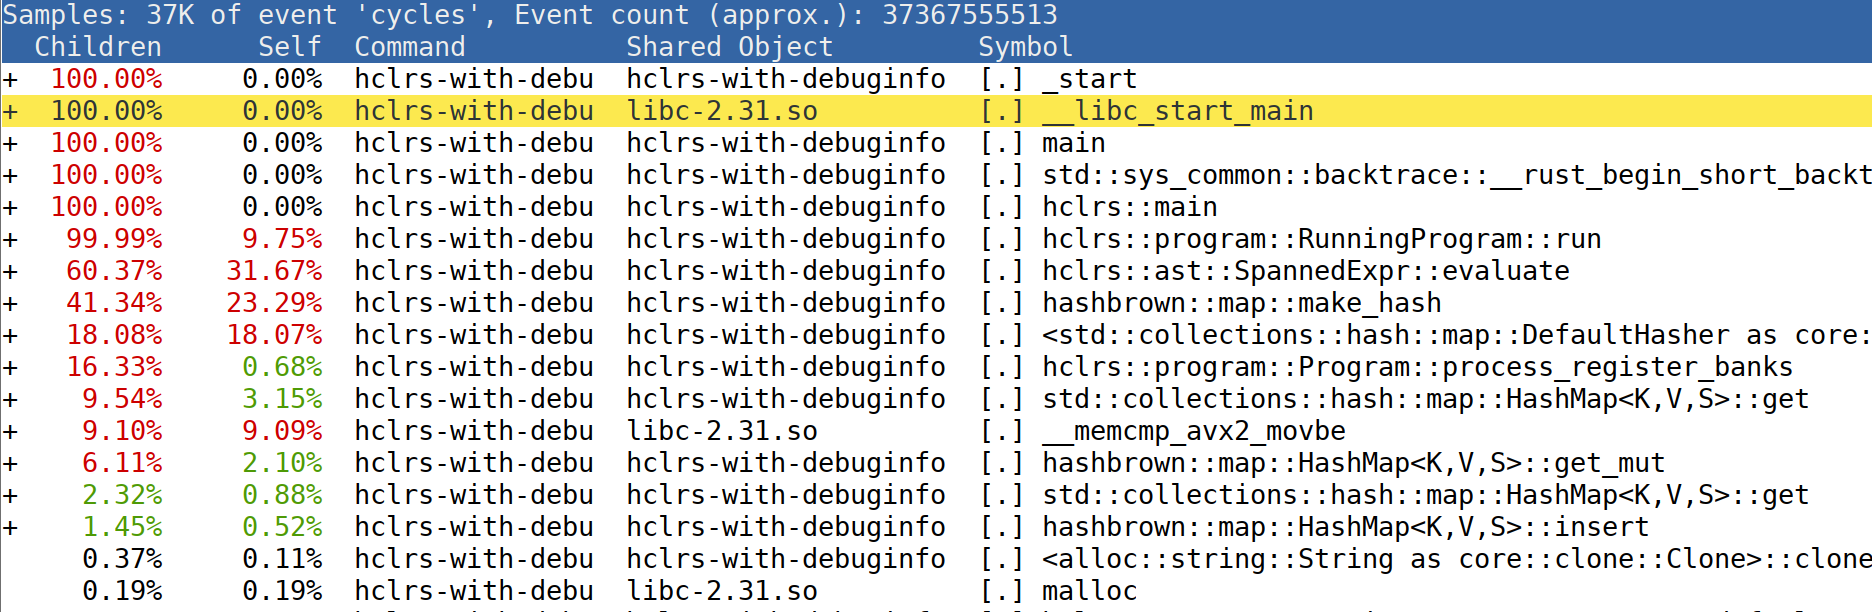
\includegraphics[width=\textwidth]{../optimization/perf-screenshot}
\end{frame}
